\chapter{ Normale Betriebsverfahren}
\pagecolor{white}
\section{Einführung}
Dieser Abschnitt enthält Checklisten und Beschreibungen für die tägliche Kontrolle und Vorflugkontrolle, sowie für die normalen Betriebsverfahren. Normale Verfahren im Zusammenhang mit Zusatzausrüstung sind im Abschnitt 9 beschrieben.


\section{Montageverfahren, Laden, Ein- und Ausbau der Akkupacks}
Die B13 lässt sich mit Hilfe einer Flächenstütze durch vier Personen auf- und abrüsten. Die Batterien können nur im abgerüsteten Zustand ein- und ausgebaut werden.

\subsection{Auf- und abrüsten}
Das Aufrüsten der B13 geschieht in folgender Reihenfolge.\\
\newline
\underline{Vorbereitungen}
\begin{itemize}
\item Transportanhänger sichern
\item alle Bolzen und Buchsen säubern und fetten
\item Trimmung kopflastig stellen, Wölbklappen auf Stellung 0 bringen und Bremsklappen entriegeln
\item Batterie in Halterung einbauen und anschließend
\item Gepäckfach einbauen

\end{itemize}

\underline{Innenflächen}
\begin{itemize}
\item Linken Hauptbolzen in das Auge des linken Innenflügels stecken
\item Linken Holmstummel bis zur Hälfte einführen
\item Rechten Hauptbolzen in das vorgesehene Auge stecken
\item Linke Innenfläche in den Rumpf stecken und beide Hauptbolzen bis zum Querkraftrohr herausziehen
\item Rechten Innenflügel in den Rumpf stecken
\item Hauptbolzenachsen zum Fluchten bringen (dies ist nur mög\-lich, wenn beide Flügel bis an den Rumpf eingeführt sind), Hauptbolzen eindrücken und sichern. Graue Markierung auf rechtem Holmstummel kann bei der Ausrichtung der Flügel helfen. (untere Kante parallel zu Holmstummeloberkante)
\item Steuerung im Rumpf anschließen und sichern - \begin{color}{red} 2x3 Anschlüsse. (L'Hotellier) \end{color} Es kann hilfreich sein, die Querruderanschlüsse im Rumpf erst nach Montage der Außenflächen anzuschließen.
\item Sicherungsschraube am Rechten Hauptbolzen lässt sich am besten einführen, wenn Hauptbolzengriff nach unten steht, danach Hauptbolzen in vorgesehene Sicherung einrasten und Sicherungsschraube mit Fokkernadel sichern.
\end{itemize}

\underline{Außenflächen}
\begin{itemize}
\item Außenflächenbolzen-Tool in das vorgesehene Loch des Außenflächenbolzens einführen
\item Außenfläche bis auf $\unit[10]{cm}$ in die Innenfläche einführen
\item Querruder anschließen und sichern \begin{color}{red} (L'Hotellier) \end{color}
\item Außenfläche vollständig einführen
\item Außenflächenbolzen von vorne in die Bohrung einführen
\item Außenflächenbolzen-Tool entfernen und mit dem federbelasteten Sicherungsstift die Außenflächen-Bolzen sichern 
\end{itemize}

\underline{Höhenleitwerk}
\begin{itemize}
\item M3-Montageschraube mit roter Kugel in den vorderen Anschlussbolzen an der oberen Seitenflossen-Vorderkante einschrauben
\item Höhenleitwerk auf beide Antriebsbolzen aufstecken und ganz nach hinten schieben
\item Montageschraube ziehen, das Leitwerk senkt sich ab und wird vom vorderen Anschlussbolzen gesichert, in dem die Montageschraube wieder losgelassen wird
\item Montageschraube herausschrauben (nach Herausschrauben, darf der Bolzen nicht mehr aus der Vorderkanten-Kontur der Seitenflosse herausstehen), Gewindeöffnung abkleben
\end{itemize}

\underline{Nachbereitungen}
\begin{itemize}
\item Düse in die Düsenaufname der Seitenflosse schieben
\item Antennenkabel an der Haube anschließen
\item Querruder, Wölbklappen, Bremsklappen, Höhenruder, Seitenruder auf Sicherung, Funktion und Freigängigkeit überprüfen
%\item Batterie in der vorgesehenen Halterung (hinter dem rechten Piloten) befestigen
\item Alle Trennstellen (Innenfläche-Außenfläche, Rumpf-Innenfläche, Seitenleitwerk-Höhenleitwerk) mit Isolierband abkleben
\end{itemize}
\begin{color}{red}
\large{\underline{Warnung}}\\
Bei den Ruderanschlüssen handelt es sich um manuelle Anschlüsse (L'Hotellier). Sie sind zu sichern (Federstecker) und vor jedem Flugbetrieb auf richtigen Anschluss und Sicherung zu kontrollieren!
\end{color}\\

Das Abrüsten geht in umgekehrter Reihenfolge wie das Aufrüsten vonstatten.

\subsection{Laden der Akkupads}

Die Betriebsanweisung zum Laden der Akkupacks ist im separaten \textbf{FES
AKKUPACKHANDBUCH} beschrieben.\\

Das Aufladen der Akkupacks kann auch optional ohne Ausbauen der Akkus erfolgen. Hierfür wurden separate Ladestecker mittig hinter den Pilotensitzen montiert. 
Die Ladegeräte werden hierfür mit speziellen Adapterkabeln mit den Ladebuchsen der B13 verbunden, die Datenkabel der Ladegeräte werden mit der vorgesehenen „CHARGE“ Buchse auf der Batteriefirewallabdeckung verbunden.\\

\begin{color}{blue}
\large{\underline{Anmerkung}}\\
Es wird empfohlen, die Akkupacks erst ein bis zwei Tage vor
dem geplanten Flug vollständig zu laden. Es soll jedoch immer genug Zeit
eingeplant werden, um einen vollständigen Ladeprozess zu garantieren!
\end{color}

\subsection{Einbau der Akkupacks in das Segelflugzeug}

\begin{color}{red}
\large{\underline{Warnung}}\\
Vor dem Einbau muss sichergestellt werden, dass beide
Akkupacks vollständig geladen sind. Beide Akkupacks müssen annähernd die
gleiche Spannung pro Zelle haben (ca. $\unit[4,16]{V}$ pro Zelle). Die Abweichung der
Gesamtspannung beider Akkupacks darf maximal $\unit[0,4]{V}$ betragen.\\
FES FLUGHANDBUCH Version 1.15 November 2016\\
Seite 17 von 34
\end{color}

Zum Einbau der Akkus wird wie folgt vorgegangen:

\begin{enumerate}
\item Akkufachabdeckung öffnen.
\item Kontrollieren, dass der Leistungsschalter ausgeschaltet ist.
\item Prüfen, dass die FCU und alle anderen Instrumente (Flugrechner, Flarm, Funk,
Transponder, PDA etc.) ausgeschaltet sind.
\item Das erste Akkupack mit dem Bedienterminal nach vorne in den Rumpf einführen und nach hinten schieben.
\item Das zweite Akkupack mit Bedienterminal nach hinten in den Rumpf einführen.
\item Ein Halteplattenpaar auf dem hinteren Akkupack mittig über dem Haltegurt positionieren und die Schraube von Hand anziehen.
\item Ein Halteplattenpaar auf dem vorderen Akkupack mittig über dem Haltegurt positionieren und die Schraube von Hand anziehen.
\item Stromkabel aus der Seitenhalterung nehmen.
\item Das kürzere Kabel mit dem $\unit[8]{mm}$ Stecker und dem SCHWARZEN Gehäuse in die mit minus markierte Buchse des vorderen Akkupacks einstecken.
\item Das längere Kabel mit dem $\unit[10]{mm}$ Stecker und dem ROTEN Gehäuse in die mit plus markierte Buchse des hinteren Akkupacks einstecken.
\item Die Stecker des Datenkabels in jeden Akkupack in den passenden DATA Anschluss einstecken.
Vor dem Einstecken vergewissern, dass die Orientierung richtig herum ist.
Die Stecker müssen gerade eingesteckt werden, ansonsten können die Pins verbogen werden.
\item “BMS Schalter” an jedem Akkupack einschalten und warten, bis der Testlauf abgeschlossen ist.
\item Akkufachabdeckung schließen.
\end{enumerate}

\section{Tägliche Kontrolle}
Vor Beginn des Flugbetriebes muss die B13 anhand der folgenden Checkliste sorgfältig überprüft werden. Insbesondere für die Ruderproben empfiehlt sich die Unterstützung durch eine zweite Person.\\
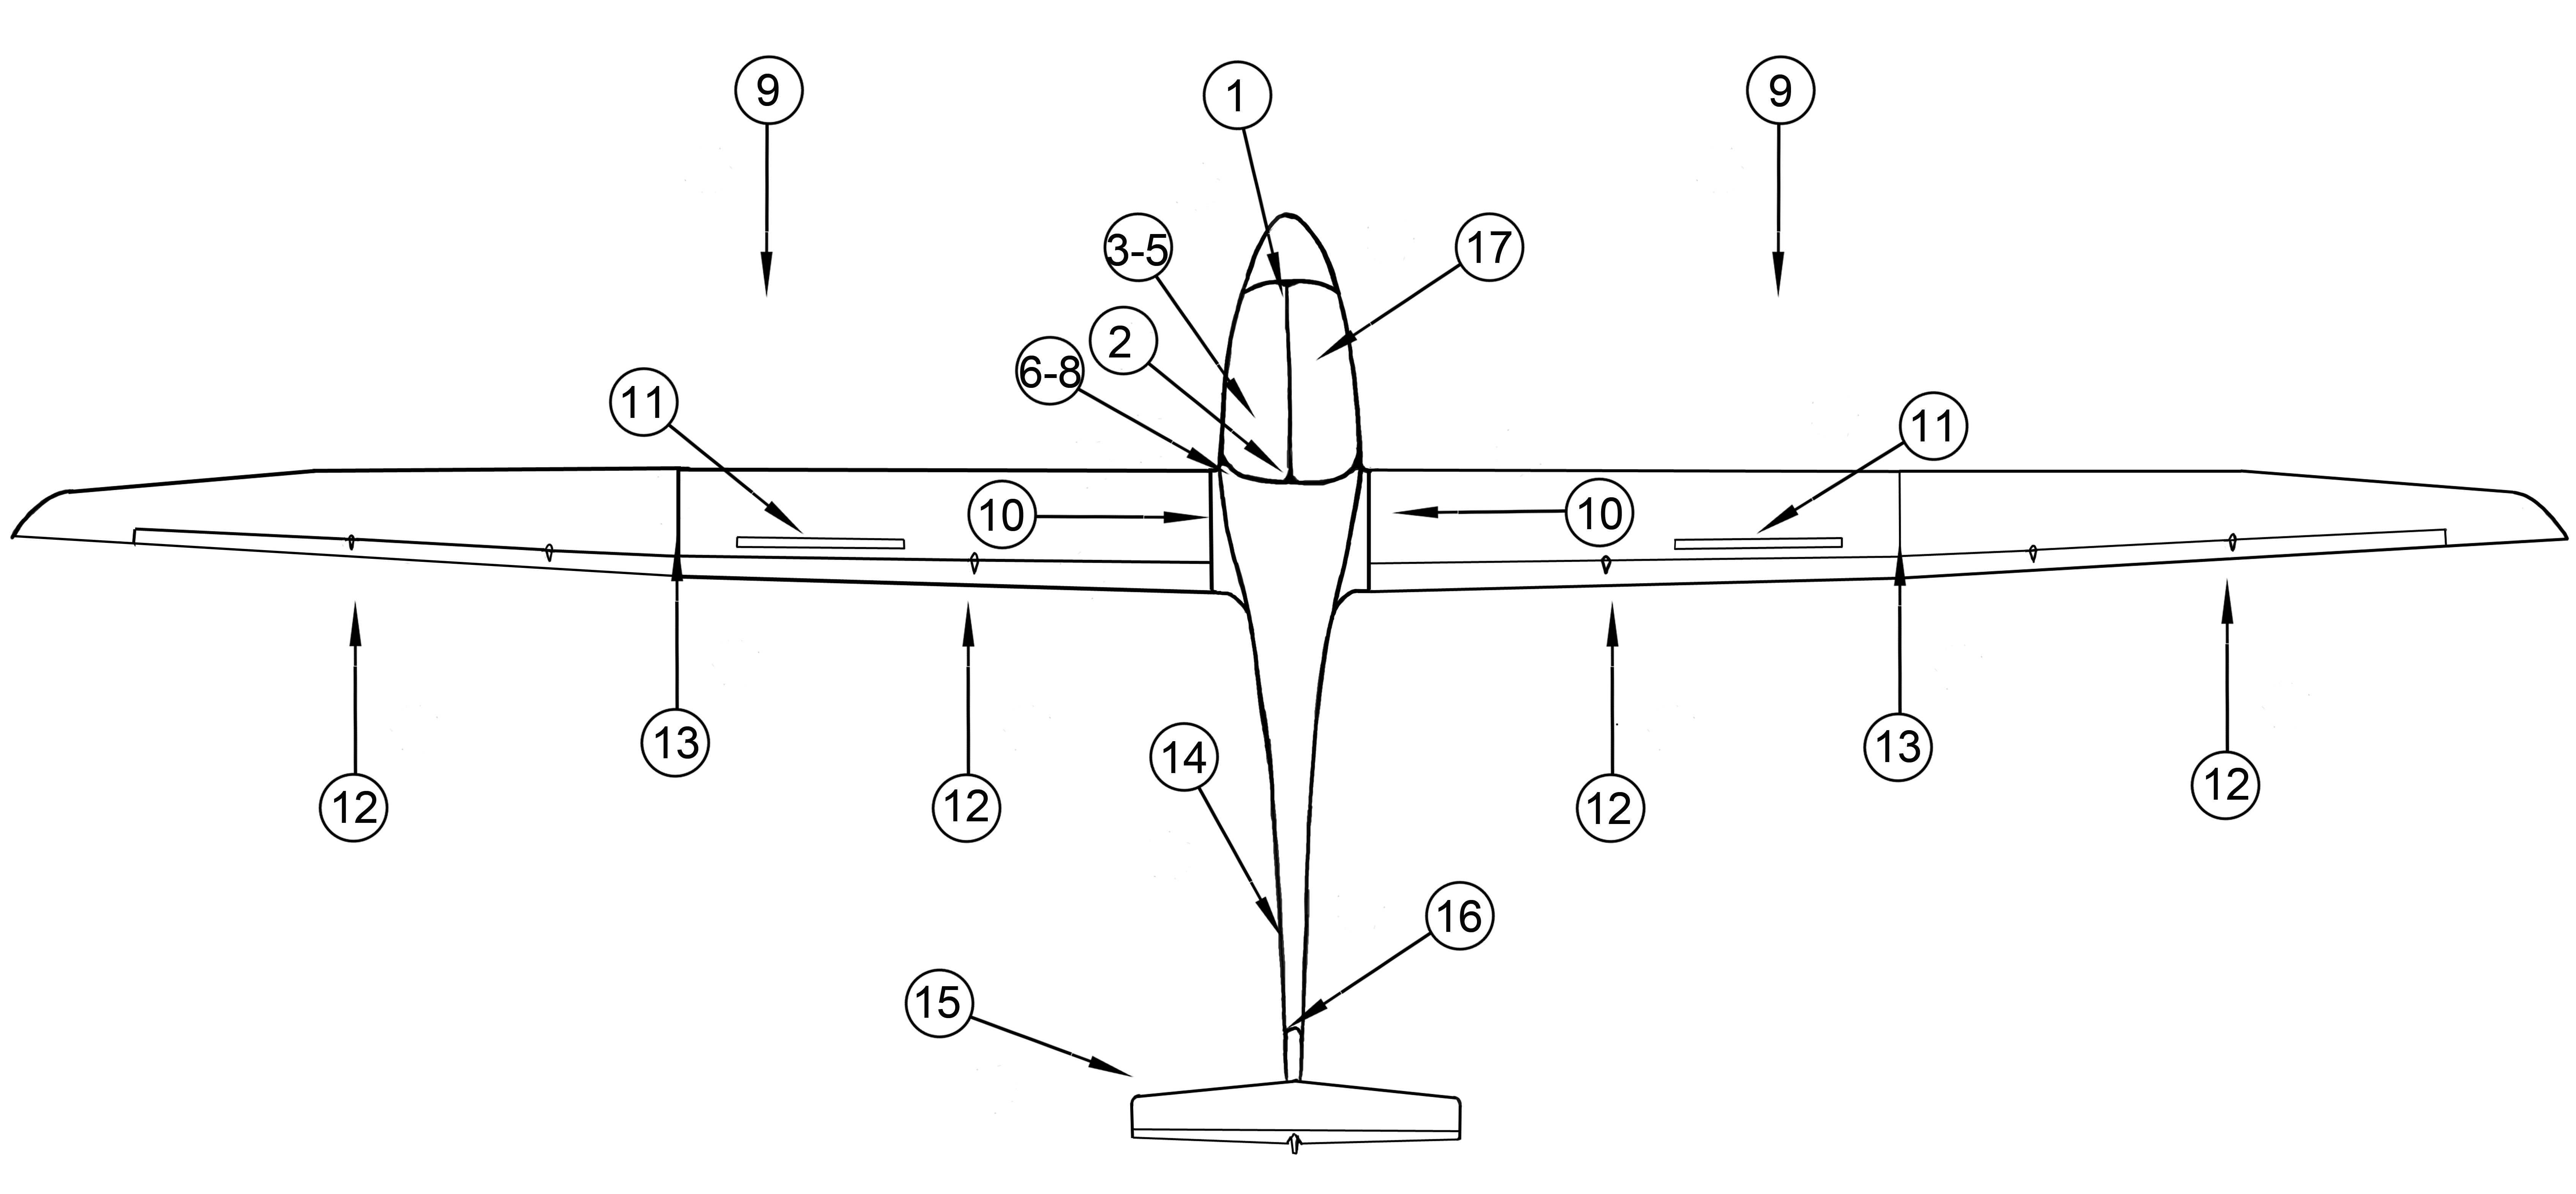
\includegraphics[width=\textwidth]{b13check.png}
\begin{enumerate}
\item Haube öffnen und Haubennotabwurf überprüfen
\item Sicherung der Hauptbolzen überprüfen
\item Fremdkörperkontrolle im gesamten Cockpitbereich
\item Freigängigkeit und Spielfreiheit aller Bedienelemente prüfen
\item Ruderprobe bei allen Rudern (Quer-, Seiten- und Höhenruder) und Klappen (Wölb- und Bremsklappe) unter Belastung durchführen. Sicherungen der Steuerung, soweit einsehbar und erreichbar, überprüfen
\item Ausklinkprobe der Schleppkupplung, auch unter Last
\item Fahrwerk und Reifen auf Beschädigungen überprüfen, Luftdruck im Reifen prüfen (auch Spornrad), Rutschmarke prüfen
\item Radbremse auf Funktion und Dichtigkeit überprüfen, Abnutzungsgrad der Bremsbeläge prüfen
\item Flügelober- und Unterseite auf Beschädigungen (Lackrisse, o.ä.) überprüfen, besonders im Bereich der Flügelwurzel
\item Flügelanschlüsse auf besonderes Spiel in den Querkraftlagern prüfen
\item Bremsklappen auf Funktion, vollständiges Schließen der Abdeckungen, Fremdkörper oder Feuchtigkeit in den Kästen überprüfen
\item Flügelklappen und Anlenkungen überprüfen (Freigängigkeit, Spielfreiheit)
\item Außenflügelanschluss - Verriegelung und Sicherung überprüfen
\item Rumpfunterseite und Leitwerksträger auf Schäden (Lackrisse, etc.) 	überprüfen, besonders im Bereich der Leitwerksanschäftung (Kuller entfernen)
\item Seiten- und Höhenleitwerk auf richtige Montage, Spiel und Beschädigungen 	überprüfen, Seilzüge des Seitenruders prüfen
\item Druckabnahmen in der Seitenflosse (Dreifachdüse) überprüfen (mit 	Fahrtmesser und Variometer)
\item Elektrisches System (Funk, Rechner) überprüfen, 	Funkprobe
\end{enumerate}

Zusätzlich ist zu Beginn jedes Flugtages und nach jedem Einbau der Akkupacks die tägliche
Kontrolle durchzufuhren. Dazu gehören mindestens die nachfolgend aufgeführten Punkte.
Werden Probleme festgestellt, so darf auf keinen Fall gestartet werden, bevor diese
Probleme nicht fachgerecht beurteilt bzw. repariert wurden.

% noch nicht vollständig
\begin{itemize}
\item Das Antriebssystem muss einer optischen Kontrolle unterzogen werden. Insbesondere der Zustand der Propellerblätter, Schlittenmechanik sowie aller Hochstromverschlüsse muss überprüft werden
\item  Füllstand des Kühlsystems muss zwischen Min und Max sein
\end{itemize}

\section{Vorflugkontrolle}
Die folgende Checkliste ist im Cockpit für beide Piloten gut sichtbar angebracht. Anhand ihrer ist vor jedem Start eine Vorflugkontrolle durchzuführen:
\begin{center}
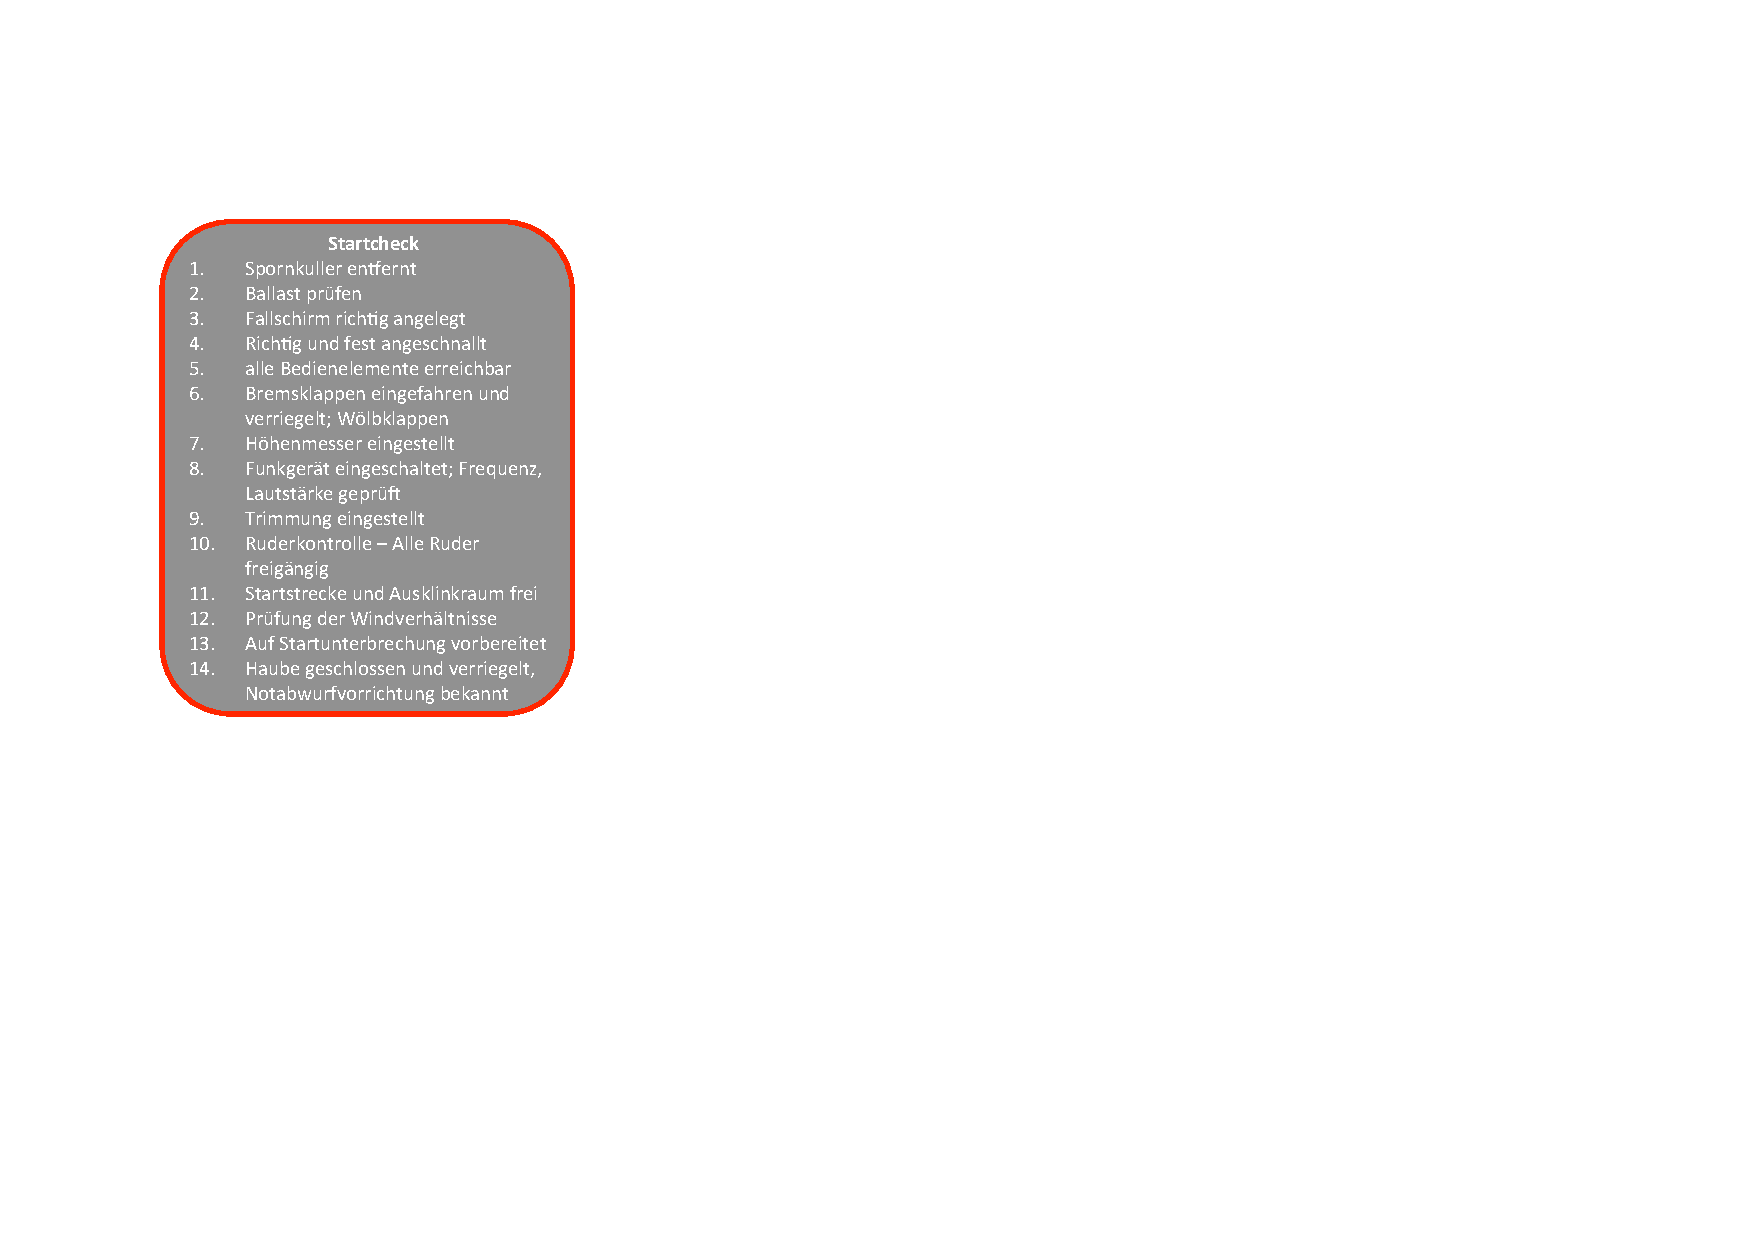
\includegraphics[width=.45\textwidth]{bilder/startcheck.pdf}
\end{center}

\subsection{Starten des Motors am Boden}

\begin{enumerate}
\item Sicherstellen, dass der \glqq ENGINE\grqq\ Schalter ausgeschaltet ist.
\item Heckkuller entfernen
\item Hochstrom Batterieanschlüsse an den Firewallboxen über"-prü"-fen. (Fester Sitz, Kabel bis zur Markierung eingesteckt)
\item CAN Bus Kabel an der Batteriefirewall auf festen Sitz über"-prü"-fen.
\item Propellerschlittensystem einschalten und warten, bis alle Statuslampen blau leuchten
\item Propeller durch Drücken des \glqq Extract\grqq-Schalters ausfahren. Warten bis alle Statuslampen grün anzeigen.
\end{enumerate}

\textbf{Tägliche Kontrolle vor dem Start: \\}
\begin{itemize}
\item Batterien geladen, korrekt eingebaut und angeschlossen?
\item Avionik Hauptschalter einschalten
\item Propellerschlittensystem einschalten
\end{itemize}

Das FES-System muss wie nachfolgend beschrieben mit einem kurzen Testlauf überprüft werden.\\

\begin{enumerate}

\item Propeller ausfahren
\item	Motorcowling entfernen
\item	Sichtkontrolle der Komponenten des Antriebes, insbesondere Propeller + Nabe, Schlittensystem + Nasenklappenmechanik, sowie aller Hochstromverschlüsse
\item	 Füllstand des Kühlsystems muss zwischen Min und Max sein
\item	 Motorcowling wieder anbauen und abkleben.
\item	Einsteigen und Haube schließen und verriegeln
\item	 Sicherstellen, dass der Propellerbereich frei ist (auch vor dem Propeller und in der Propellerebene)
\item	FCU einschalten
\item	Leistungsschalter einschalten.
\item	Die Kühlwasserpumpe muss leise hörbar anlaufen. Ein ungleichmäßiges ratterndes Geräusch deutet auf Luft im Kühl"-wassersystem hin. In diesem Falle Kühlsystem entlüften
\item	Ca. 8 Sekunden warten, bis alle Akkusymbole im Display angezeigt werden
\item	Radbremse Betätigen oder Flugzeug anderweitig vom Wegrollen hindern
\item	 Motor starten und danach kurzenTestlauf durchführen. Im Standlauf sind Drehzalen bis $\unit[3000]{u/min}$ erprobt. Der Motorlauf muss frei von starken Vibrationen sein

\begin{color}{red}
\large{\underline{Warnung}}\\
Beim Abschalten des Motors wird auch die Kühlung abgeschaltet. Der dadurch verursachte Temperaturanstieg kann den Motor beschädigen!
\end{color}\\

\item	Sicherstellen, dass die Motorbremse funktioniert.
\item	Leistungsschalter ausschalten.
\item	Propeller einfahren
\item	FCU, Propellerschlittensystem und Avionik ausschalten, wenn nicht gleich gestartet werden soll.
\end{enumerate}


\section{Normalverfahren und empfohlene Geschwindigkeiten}

\subsection{Windenstart}
Während des Windenstarts müssen der Propeller und alle Klappen eingefahren sein. Die Kühlluftklappe wird im ausgefahrenen Zustand durch das Schleppseil zerstört.\\

Die höchstzulässige Geschwindigkeit im Windenschlepp beträgt $V_W=\unit[120]{\frac{km}{h}}$. Die normale Schleppgeschwindigkeit beträgt $\unit[110]{\frac{km}{h}}$ (bei maximaler Abflugmasse $\unit[120]{\frac{km}{h}}$) und sollte nicht um mehr als $\unit[10]{\frac{km}{h}}$ unterschritten werden.\\
Vor dem Start ist die Trimmung neutral bis leicht kopflastig zu stellen. Beim Anrollen wird bis zum Erreichen von ausreichend Querruderwirkung die Wölbklappenstellung $-2$ empfohlen, danach sollte auf die Wölbklappenstellung $+1$ umgewölbt werden.\\
Das Windenseil sollte mit einer Sollbruchstelle ausgestattet sein, die eine maximalen Bruchlast von $\unit[1000]{daN}$ (schwarz) erreicht. \\
\newline
\begin{color}{red}
\large{\underline{Warnung}}\\
Von \underline{Rückenwindschlepps} an schwachen Schleppwinden, besonders in Zusammenhang mit hohen Außentemperaturen wird ausdrücklich abgeraten.
\end{color}\\
\newline
\begin{color}{red}
\large{\underline{Warnung}}\\
Während des Windenstarts darf das Antriebssystem nicht ausgefahren und gestartet werden! Bevor das Antriebssystem ausgefahren und der Motor gestartet werden darf, muss das Schleppseil ausgeklinkt werden!
\end{color}\\
\newline
\begin{color}{forestgreen}
\large{\underline{Wichtiger Hinweis}}\\
Vor dem Start müssen beide Piloten ihre Sitzposition und die Erreichbarkeit der 	Bedienelemente überprüfen. Die Sitzposition, besonders mit einem Sitzkissen, muss so sein, dass ein Zurückrutschen beim Anschleppen oder im steilen Steigflug ausgeschlossen ist. Ebenso ist das sichere Einrasten der Pedalverstellungen zu überprüfen.
\end{color}\\
\newline
\newline
\begin{color}{forestgreen}
\large{\underline{Wichtiger Hinweis}}\\
Querneigung beachten!
\end{color}\\
\subsection{Flugzeugschlepp}
Vor dem Start muss die FCU immer eingeschaltet werden. Es muss sichergestellt sein, dass der Leistungsschalter ausgeschaltet ist, wenn sich Personen im Propellerbereich befinden, um das Schleppseil einzuklinken. Während des Schlepps muss der Leistungsschalter ausgeschaltet sein!\\

\begin{color}{red}
\large{\underline{Warnung}}\\
Während des Flugzeugschlepps darf das FES System nicht
gestartet werden!
\end{color}\\

Die höchstzulässige Schleppgeschwindigkeit beträgt $V_T=\unit[160]{\frac{km}{h}}$. Die normale Schleppgeschwindigkeit liegt bei $\unit[110-130]{\frac{km}{h}}$. \\
Auch für den Flugzeugschlepp wird die Schwerpunktkupplung auf der Rumpfunterseite verwendet. Es sollte daher ein ausreichender Übungsstand bei F-Schlepps an Schwerpunktkupplungen vorliegen. Das Schleppseil sollte eine Bruchlast von $\unit[1000]{daN}$ (schwarz) erreichen und eine Länge zwischen $\unit[30]{m}$ und $\unit[60]{m}$ haben.\\
Vor dem Start ist die Trimmung in Neutralstellung zu bringen. Die Wölbklappen befinden sich in der Stellung $-2$. Sobald ausreichend Querruderwirkung vorhanden ist, wird vorsichtig auf $+1$ umgewölbt. Das Abheben erfolgt in dieser Wölbklappenstellung. \\
Bei Überlandschlepps und höheren Schleppgeschwindigkeiten kann auch auf die $0$ oder  $-1$ Stellung umgewölbt werden.\\
Das Fahrwerk kann während des Flugzeugschlepps in sicherer Höhe vorzugsweise vom Copiloten eingefahren werden.\\
\newline
\begin{color}{red}
\large{\underline{Warnung}}\\
Nicht das Schleppflugzeug übersteigen!
\end{color}\\
\newline
\begin{color}{forestgreen}
\large{\underline{Wichtiger Hinweis}}\\
Es wird empfohlen ein längeres Schleppseil aufgrund der außermittigen Sitzposition zu verwenden, um Schiebeflugzustände im F-Schlepp zu 	vermeiden. Jeder Sitz sollte zusätzlich mit einem eigenen Haubenfaden ausgestattet sein. Bei negativen Wölbklappenstellungen kann das Schleppflugzeug schnell unter dem Haubenrahmen verschwinden.
\end{color}\\
\newline
\begin{color}{forestgreen}
\large{\underline{Wichtiger Hinweis}}\\
Querneigung beachten!
\end{color}\\
\newline
\begin{color}{blue}
\large{\underline{Anmerkung}}\\
Es empfiehlt sich, vor dem Anrollen die Radbremse leicht anzuziehen, damit ein	Überrollen des Schleppseils vermieden wird. 
\end{color}\\
\newline
\begin{color}{blue}
\large{\underline{Anmerkung}}\\
Die Schleppmaschine sollte aufgrund des hohen Abfluggewichtes der B13 ausreichend motorisiert sein.
\end{color}\\

\subsection{Rollverfahren}
\begin{color}{red}
\large{\underline{Warnung}}\\
Rollen ist mit dem Antriebsystem als Hilfsantrieb verboten!
\end{color}

\subsection{Eigenstart und Steigflug}
\begin{color}{red}
\large{\underline{Warnung}}\\
Ein Eigenstart mit der B13 ist nicht zugelassen!
\end{color}\\
\newline

\subsection{Freier Flug}
Die B13 zeigt bei allen Schwerpunktlagen, Beladungszuständen, Wölbklappenstellungen und Fluggeschwindigkeiten ein angenehmes Flugverhalten. Unangenehme Eigenschaften wurden bisher nicht ermittelt. Im freien Geradeausflug kann man alle Ruder freigeben, ohne daß das Flugzeug dazu neigt eine neue Fluglage einzunehmen. Um einen schiebefreien Flug zu erreichen, sollte jeder Sitz über einen eigenen Faden verfügen.\\
\newline
Der Trimmbereich geht von ca. $\unit[80]{\frac{km}{h}}$ bis zu über $\unit[220]{\frac{km}{h}}$. Die Kurvenwechselzeiten aus $45^{\circ}$ - Kurven liegen bei ungefähr $\unit[4]{s}$.\\

\begin{itemize}
\item \textbf{Gebrauch der Wölbklappen}\\
Die optimale Stellung der Wölbklappen hängt stark von der Flächenbelastung ab. Für eine Flächenbelastung von $\frac{G}{S}=\unit[396]{\frac{N}{m^2}}$ sind die Geschwindigkeits- und Gleitzahlpolare in Kapitel 5.3.2 und 5.3.3 abgebildet. 
Es sollte darauf geachtet werden, dass ein ruckartiges Betätigen der Wölbklappen eventuell ein Durchsacken oder Wegsteigen bewirken könnte. Dieses Verhalten kann besonders in Bodennähe zu kritischen Situationen führen. Die Wölbklappen sollten daher immer langsam und kontinuierlich betätigt werden. 
\item \textbf{Überzieheigenschaften}\\
Der überzogene Flugzustand äußert sich bei der B13 durch weiche Ruder, Taumeln, Nicken, Schütteln und schließlich dem Sackflug. Bei diesen hohen Anstellwinkeln muss davon ausgegangen werden, dass die Fahrtmesseranzeige stark durch die Strömungsablösungen am Rumpf beeinflusst wird und daher keine richtigen Fluggeschwindigkeiten anzeigt.  Der überzogene Flugzustand oder gar ein Abkippen über eine Fläche kann durch Nachlassen des Höhensteuers und – wenn erforderlich – durch Gegenseitenruder beendet werden. 
\item \textbf{Schnellflug}\\
Für den Schnellflug sind die Klappenstellungen $0$, $-1$ und $-2$ vorgesehen. Es sollte darauf geachtet werden, dass die $V_{NE} = \unit[220]{\frac{km}{h}}$  und die maximalen Abfanglastvielfachen nicht überschritten werden. Weiterhin dürfen ab der Manö"-ver"-geschwindigkeit von $V_A = \unit[160]{\frac{km}{h}}$ nur noch $\frac{1}{3}$ der Ruderausschläge gegeben werden. 

\end{itemize}

Da das Propellersystem in Segelflugkonfiguration vollständig eingeklappt ist, gibt es keine Änderungen zur bisherigen Konfiguration der B13.

Während des Fluges muss die FCU immer eingeschaltet sein.

\newpage
\subsection{Reise- und Steigflug mit laufendem Motor}
Das Antriebssystem ist geeignet für langen kontinuierlichen Reiseflug bei geringer Leistung oder schnelles Steigen bei hoher Leistung.\\

\textbf{Motor anlassen während des Fluges:}
\begin{enumerate}
\item Sicherstellen, dass alle angezeigten Daten der FCU im Normalbereich sind (FCU muss während des gesamten Fluges eingeschaltet sein).
\item Propellerschlittensteuerung einschalten
\item Propeller ausfahren. Alle Statuslampen müssen Grün anzeigen. Canopy Open Warnung darf nicht mehr auf der FCU angezeigt werden.
\item Leistungsschalter einschalten.
\item Sicherstellen, dass grüne LED leuchtet (LED links unten), Spannung überprüfen
\item Leuchtet die grüne LED nicht oder blinkt die rote LED, startet der Motor nicht. 
\item Zum Motorstart den Leistungsdrehregler vorsichtig im Uhrzeigersinn drehen
\end{enumerate}

Für den Horizontalflug ist eine Leistungseinstellung von ca.
\unit[8]{kW} zu nutzen, für den
Steigflug mehr. Die Steigrate ist abhängig von Masse, Geschwindigkeit, Wölbklappenstellung, etc.
Die verfügbare maximale Leistung reduziert sich in Folge des Spannungsabfalls, bzw.
durch die Entladung der Akkupacks. Die maximale Leistung kann nur solange genutzt werden bis einer der Temperaturwerte den gelben Bereich erreicht. (Motor $\unit[100]{^\circ C}$, Controller $\unit[60]{^\circ C}$, Akkupacks $\unit[45]{^\circ C}$)!\\

Genaue Informationen zur FCU sind im FES FCU INSTRUMENTENHANDBUCH zu finden.\\

\begin{color}{blue}
\large{\underline{Anmerkung}}\\
Leistung in der Thermik reduzieren, in sinkender Luft erhöhen.\\
Bei niedrigen Spannungen darf keine hohe Stromstärke verwendet werden (unter
$\unit[95]{V}$).\\
Wenn möglich sollte mit niedriger Leistungseinstellung geflogen werden, da dort das
Antriebssystem am effizientesten ist.\\
Während dem motorgetriebenen Flug muss die FCU eingeschaltet sein. Ist der Motor
abgeschaltet, soll auch der Leistungsschalter ausgeschaltet werden.
\end{color}

\subsection{Propeller anhalten mit elektrischer Bremse}
Um den Propeller mit der elektrischen Bremse anzuhalten, muss der Leistungsdrehregler entgegen dem Uhrzeigersinn in einer Bewegung auf null-Leistung gedreht werden, sodass die Leistungsanzeige auf dem Display rot blinkt.

\newpage
\subsection{Landeanflug}
An dem Punkt \glqq Position\grqq\ wird folgende Lande-Checkliste durchgeführt:
\newline
\begin{center}
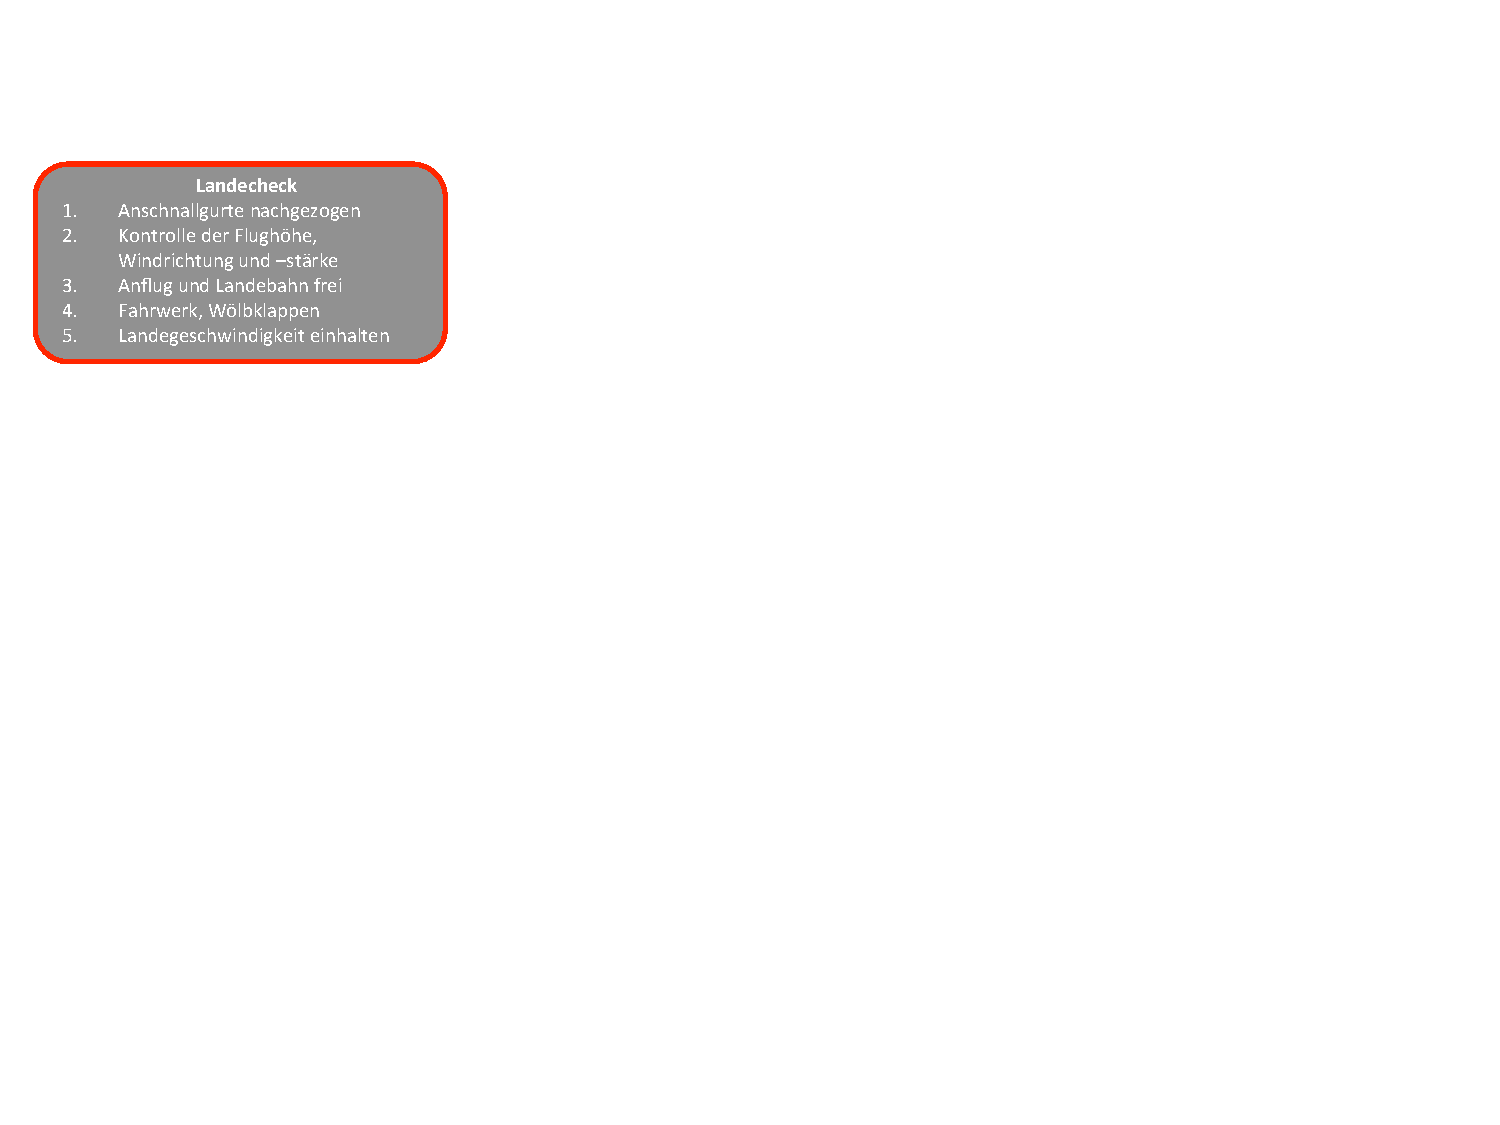
\includegraphics[width=.45\textwidth]{bilder/landecheck.pdf}
\end{center}

Vergewissern Sie sich, dass der \glqq Engine\grqq-Schalter ausgeschaltet ist und der Propeller eingezogen ist.\\

Die normale Anfluggeschwindigkeit für die maximale Masse mit voll ausgefahrenen Bremsklappen und ausgefahrenem Fahrwerk liegt bei $\unit[100]{\frac{km}{h}}$ (gelbes Dreieck auf dem Fahrtmesser).\\
Die Wirkung eines Seitengleitfluges ist gering. Die Wirkung der dreistöckigen Bremsklappen ist mäßig. (Gleitzahl bei ausgefahrenen Bremsklappen ca. $7,2$) \\
Für kurze Landungen über ein Hindernis wird es erfahrenen Piloten empfohlen, schon in größerer Höhe die Fahrt zu reduzieren, da die Wirkung des Bodeneffektes beachtlich ist.\\
Die B13 sollte mit voll gezogenem Höhenruder in 2-Punkt-Lage aufgesetzt werden, Spornradlandungen sind auch problemlos mög"-lich. Nach dem Aufsetzen sollte auf die Wölbklappenstellung $-2$ umgewölbt werden, um die Querruderwirkung bis zum Stillstand aufrecht zu erhalten. Es empfiehlt sich, den Copiloten dabei die Bremsklappen in der gewünschten Stellung festhalten zu lassen, um ein Hereinfallen dieser zu verhindern. \\
Die Radbremse wird bei vollem Ausfahren der Bremsklappen mitbetätigt und ist gut wirksam.
Das Fahrwerk muss immer ausgefahren werden, da es den Piloten und die Flugzeugstruktur vor starken Landestößen schützt.\\
\newline
\begin{color}{blue}
\large{\underline{Anmerkung}}\\
Aufgrund der Sitzposition sollte die Platzrunde in Richtung des fliegenden Luftfahrzeugführers bevorzugt werden, da die Sichtverhältnisse zur anderen Seite eingeschränkt sind.
\end{color}\\
\newline
\begin{color}{forestgreen}
\large{\underline{Wichtiger Hinweis}}\\
Der Seitengleitflug ist nur wenig wirksam und deshalb als Landehilfe nur bedingt geeignet.
\end{color}\\
